\section{灵敏度分析与稳健性讨论}
\label{sec:sensitivity}

本文从局部参数和边界闭合两个层面考察终点变化。局部分析选取换热系数$h$、传质系数$h_m$、扩散率整体尺度$D$和边界映射系数$\beta$，在其余条件不变时分别施加$\pm10\%$扰动；其中$D$表示完整经验扩散率的乘数，$C_{\mathrm{eq}}=\beta Y$。由于题目未给出参数分布，以下结果均为确定性情景。

\subsection{指标定义与试验设计}

以临界时间$t_*$为响应量，定义参数$p$的有符号无量纲局部灵敏度系数
\begin{equation}
S_p=\left.\frac{\partial\ln t_*}{\partial\ln p}\right|_{p_0}
\approx\frac{t_*(1.1p_0)-t_*(0.9p_0)}{0.2t_*(p_0)}.
\label{eq:sensitivity-index}
\end{equation}
$S_p<0$表示增大该参数会缩短干燥时间，$|S_p|$越大表示局部影响越强。式\eqref{eq:sensitivity-index}使用对称差分，可同时利用正、负扰动并降低单侧差分偏差。每个扰动场景均从相应原始初态完整重算，重新搜索全域阈值事件，而不是在基准终点附近线性外推。

表\ref{tab:local-sensitivity}给出两问的重算结果。问题三、四的基准时间分别为$57.4740$ h和$51.0920$ h。

\begin{table}[htbp]
  \caption{临界时间局部灵敏度}
  \label{tab:local-sensitivity}
  \centering
  \begin{tabular}{cclrrrr}
    \toprule
    问题 & 参数 & 扰动含义 & $t_*(-10\%)$/h & $t_*(p_0)$/h & $t_*(+10\%)$/h & $S_p$ \\
    \midrule
    \multirow{4}{*}{问题三}
      & $h$ & 换热强度 & 57.4828 & 57.4740 & 57.4669 & $-0.0014$ \\
      & $h_m$ & 表面传质 & 58.2099 & 57.4740 & 56.8967 & $-0.1142$ \\
      & $D$ & 内部扩散 & 63.1322 & 57.4740 & 52.8666 & $-0.8931$ \\
      & $\beta$ & 平衡边界 & 57.3721 & 57.4740 & 57.5949 & $+0.0194$ \\
    \midrule
    \multirow{4}{*}{问题四}
      & $h$ & 换热强度 & 51.1001 & 51.0920 & 51.0855 & $-0.0014$ \\
      & $h_m$ & 表面传质 & 51.3832 & 51.0920 & 50.8712 & $-0.0501$ \\
      & $D$ & 内部扩散 & 56.0919 & 51.0920 & 47.0123 & $-0.8885$ \\
      & $\beta$ & 平衡边界 & 50.9893 & 51.0920 & 51.2233 & $+0.0229$ \\
    \bottomrule
  \end{tabular}
\end{table}

\subsection{边界闭合的宽情景检验}

$\pm10\%$扰动只反映$\beta=1$附近的局部斜率，对空气水分量到药材平衡含水率的定义差异覆盖不足。为此，将$\beta$扩展到$0.5$、$2.0$和$2.8$，沿用相同环境、物性和事件判据完整重算。长期平台水分量为$Y=0.0499875$，结果见表\ref{tab:boundary-closure-scenarios}。

\begin{table}[htbp]
  \caption{平衡边界闭合的宽情景}
  \label{tab:boundary-closure-scenarios}
  \centering
  \begin{tabular}{crrr}
    \toprule
    $\beta$ & 长期$C_{\mathrm{eq}}$ & 问题三$t_*$/h & 问题四$t_*$/h \\
    \midrule
    0.5 & 0.0250 & 57.0650 & 50.7478 \\
    1.0 & 0.0500 & 57.4740 & 51.0920 \\
    2.0 & 0.1000 & 61.2846 & 55.0980 \\
    2.8 & 0.1400 & 85.6727 & $>72$\textsuperscript{a} \\
    \bottomrule
    \multicolumn{4}{l}{\footnotesize \textsuperscript{a}72 h时$C_{\max}=0.15185$；半径观测在此处结束。} \\
  \end{tabular}
\end{table}

当长期$C_{\mathrm{eq}}$由0.05提高到0.10时，两问终点分别延后3.81 h和4.01 h；提高到0.14后，问题三终点增至85.67 h，问题四在72 h半径观测范围内仍未达标。若长期$C_{\mathrm{eq}}\ge0.15$，在持续平台边界下模型将趋向不低于阈值的平衡状态，严格停机事件不再出现。基准点附近较小的$S_\beta$只说明局部扰动影响有限，边界映射本身仍是长期预测的主要结构来源。表中数值是给定$\beta$下的条件结果，不表示其概率范围。

\subsection{参数敏感性排序与机理解释}

图\ref{fig:sensitivity-risk}(a)(b)展示正、负扰动引起的终点相对变化，图\ref{fig:sensitivity-risk}(c)进一步保留影响方向。两问均有
\begin{equation}
|S_D|>|S_{h_m}|>|S_{\beta}|>|S_h|.
\end{equation}
扩散率尺度的$S_D$约为$-0.89$，即在基准点附近，扩散率提高$1\%$大致对应临界时间降低$0.89\%$；它是四个局部参数中影响最大的一个。这与临界阶段仍存在显著内部含水率梯度的结果一致。$h_m$位居第二，但问题四中的$|S_{h_m}|$由问题三的$0.1142$降至$0.0501$：收缩缩短内部路径并提高面积体积比后，终点对外膜传质的局部响应减弱。

$S_h$在两问中均约为$-0.0014$，原因是终点阶段温场已接近环境平台。$S_\beta>0$，增大$\beta$会提高等效平衡含水率、减小表面排湿驱动力。温度依赖影响早期扩散率演化，而终点对$h$本身的局部响应很弱，二者对应不同阶段。

正负扰动的响应还具有轻微不对称性。例如问题三中$D$降低$10\%$使终点延后$9.8447\%$，而提高$10\%$只使其提前$8.0165\%$；问题四对应$+9.7859\%$和$-7.9850\%$。这是变物性、时变边界与事件判停共同造成的非线性，局部灵敏度系数适用于基准点邻域。

\begin{figure}[htbp]
  \centering
  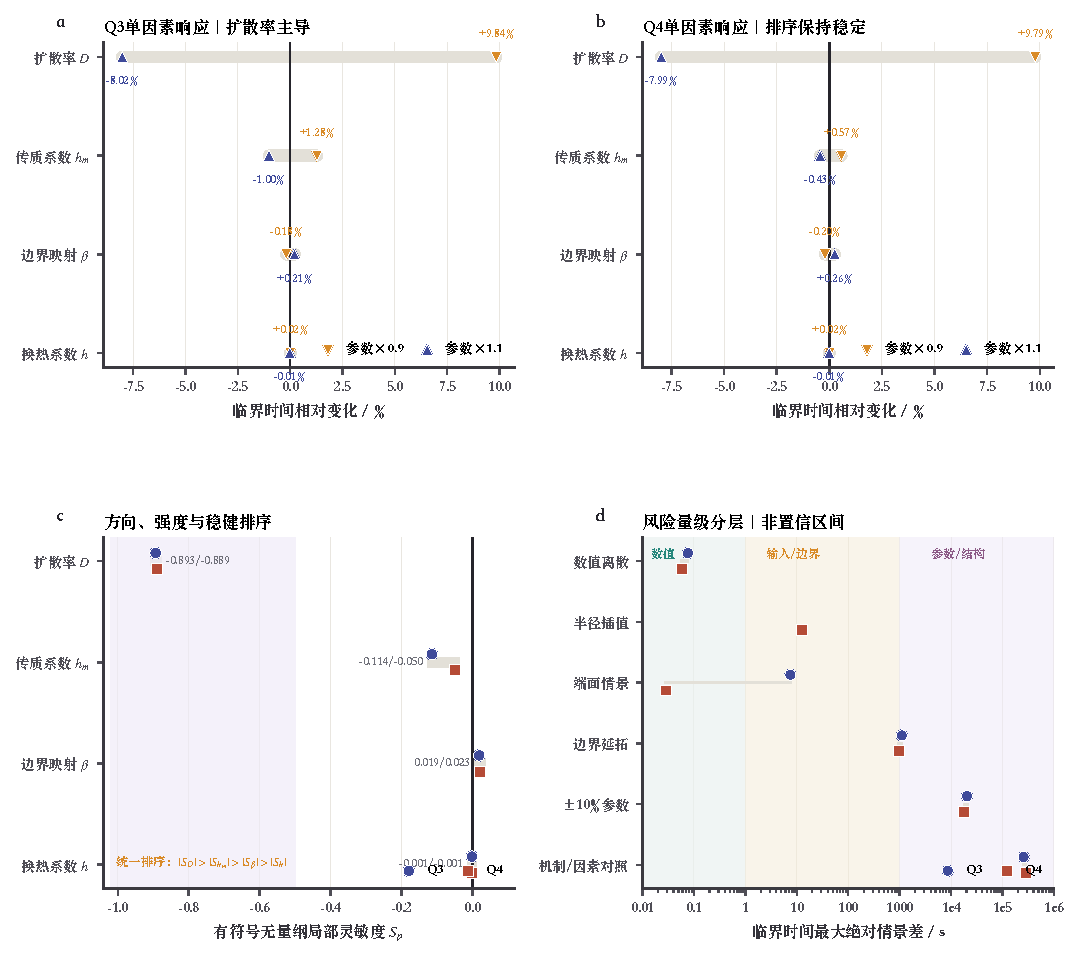
\includegraphics[width=0.98\textwidth]{figures/fig07_sensitivity_risk.pdf}
  \caption{终点灵敏度与风险层级}
  \label{fig:sensitivity-risk}
\end{figure}

图\ref{fig:sensitivity-risk}(a)(b)在扰动端点标出终点相对变化，$D$的正负扰动存在约1.8个百分点的不对称；(c)保留两问数值和统一排序；(d)区分数值、输入/边界及参数/结构三类量级。$D$的排序针对基准附近的四个局部参数，边界闭合的宽情景则刻画模型口径改变后的终点变化。

\subsection{情景稳健性与误差层级}

参数扰动之外，本文还比较输入延拓、半径插值、端面条件和模型结构情景。图\ref{fig:sensitivity-risk}(d)以对数轴给出临界时间最大绝对差：纯数值离散约为$10^{-1}$ s量级，问题四半径插值为$12.61$ s，端面配对情景约为$7.49$ s和$0.028$ s，环境延拓约为$10^3$ s，$\pm10\%$参数扰动约为$2\times10^4$ s，而机制或因素对照可达$10^5$ s量级。不同层级相差数个数量级，说明继续增加终点求根小数位不会弥补边界和结构假设的不确定性。

具体而言，4 h后若保持末次观测而非采用3--4 h均值，问题三、四分别提前约18.28 min和16.07 min；问题四将半径线性插值改为PCHIP，终点仅提前12.61 s。冻结扩散率中的温度因子会把问题三终点推迟至$128.9902$ h，说明该经验模型中的温度依赖会影响完整过程。这一消融远离基准模型，用于解释机制，与$\pm10\%$局部参数扰动分开比较。

若用于实际预测，应优先通过实验校准$D(C,T)$、平衡含水率关系和表面传质系数，并补充长期环境与端面边界信息。当前网格和时间容差对终点的影响已小于这些物理输入。
